 % -----------------------------------------------
% Template for SMC 2009
%     smc2009.sty -> style file
% Last modified by Fabien Gouyon (smc2009@inescporto.pt)
% Modified by Juan P. Bello (ismir2008-papers@ismir.net)
% By Rainer Typke (ismir07.rainer@safersignup.com)
% Based on the 2004 template by Eloi Batlle.
% -----------------------------------------------

\documentclass{article}
\usepackage{smc2009,amsmath}
% To use when using pdflatex
\usepackage{graphicx}
\usepackage{url}     
\usepackage{hyperref}  
      
\newenvironment{packed_item}{
\begin{itemize}
  \setlength{\itemsep}{1pt}
  \setlength{\parskip}{0pt}
  \setlength{\parsep}{0pt}
}{\end{itemize}}

\newenvironment{packed_enumerate}{
\begin{enumerate}
  \setlength{\itemsep}{1pt}
  \setlength{\parskip}{0pt}
  \setlength{\parsep}{0pt}
}{\end{enumerate}}
% To use when using latex, dvips and ps2pdf
% \usepackage[dvips]{graphicx}

% Title.
% ------
%\title{a layered approach to sound spatialization - concepts and examples}
\title{A stratified approach for sound spatialization}
% IMPORTANT NOTICE:
% Reviews are double-blind
% Authors will not be informed of who reviews their papers, and author names will be concealed from the reviewers 
% Please avoid evident self references in the text

% Authors' names must be omitted from title page (or listed as �name(s) omitted for submission�)


% Single address
% To use with only one author or several with the same address
% ---------------
\oneauthor
   {Nils Peters$^{a}$, Trond Lossius$^{b}$, Jan Schacher$^{c}$, Pascal Baltazar$^{d}$, Charles Bascou$^{e}$, Timothy Place$^{f}$}
   {$^{a}$ CIRMMT, McGill University, Montr\'eal, nils.peters@mcgill.ca\\ $^{b}$ BEK - Bergen Center for Electronic Arts, trond.lossius@bek.no\\ $^{c}$ ICST, Zurich University of the Arts, jan.schacher@zhdk.ch \\ $^{d}$ GMEA - National Centre for Musical Creation of Albi, pb@gmea.net\\ $^{e}$ GMEM - National Centre for Musical Creation of Marseille, charles.bascou@gmem.org \\ $^{f}$ Cycling~'74, tim@cycling74.com} 
%TODO : Could be nice to put GMEA and GMEM entire names, which are : GMEA/M National Centre for Musical Creation of Albi/Marseille. I know this is long, but at least the cities would be nice...
 

%{CIRMMT, McGill University, Montr\'eal$^{a}$ --- BEK - Bergen Center for Electronic Arts \\Zurich School of Music, Drama and Dance --- GMEA --- GMEM --- Cycling~'74 \\ nils.peters@mcgill.ca trond.lossius@bek.no jan.schacher@zhdk.ch \\ pb@gmea.net charles.bascou@gmem.org tim@cycling74.com}

% Two addresses
 %--------------
%\threeauthors
%  {Nils Peters} {School \\ Email}
%  {Second author} {Company \\ Email}
%  {Third author} {Company \\ Email}
% Three addresses
% --------------
%\threeauthors
%  {First author} {School \\ Email}
%  {Second author} {Company \\ Email}
%  {Third author} {Company \\ Email}

\begin{document}
%    
\sloppy
\maketitle
%

\permission

\begin{abstract}  
We propose a multi-layer structure to mediate essential components in sound spatialization. This approach will facilitate artistic work with spatialization systems, a process which currently lacks structure, flexibility, and interoperability. 
\end{abstract}

\section{Introduction}\label{sec:introduction}         
The improvements in computer and audio equipment in recent years make it possible to experiment more freely with resource-demanding sound synthesis techniques such as spatial sound synthesis, also known as spatialization.
%TODO : maybe clarify next sentence... Pascal isn't really able to understand it... "For seeking", is that English ?
For seeking new means of expression, different spatialization applications should be readily combined and accessible for both programmatic and user interfaces. % and/or other controllers. %e.g. a generative mapping of a granular synth output to different spatial renderer from one common user interface, while also streaming spatial encoded audio to the internet. 
Furthermore, 
%The goal of any spatialization
%rendering is it only the rendering system, or control/rendering ?
%system is to facilitate or empower the creative use of the spatial medium for a sonic artist. 
quantitative studies on spatial music (e.g. \cite{otondo2008ctu}) remind us that there are great individual and context-related differences in the compositional use of spatialization and that there is no one spatialization system that could satisfy every artist. %that the compositional use of spatialization techniques varies strongly across composers and musical context.    
% TODO Tim thinks we can drop this next sentence, as it is redunant with the following sentences
% For instance, the requirements of a computer aided spatialization system may vary between a fixed-media composition, an art-installation, and a live diffusion performance. 
In an interactive art installation, the real-time quality of a spatial rendering system in combination with the possibility to control spatial processes through a multi-touch screen can be of great importance. In contrast, the paramount features in a performance of a fixed-media composition may be multichannel playback and the compensation of non-equidistant loudspeakers (in terms of sound pressure and time delays). Additional scenarios may require binaural rendering for headphone listening, multichannel recording, up and down mixing, or a visual representation of a sound scene.  
Moreover, even during the creation of one spatial art work, the importance of these requirements may change throughout different stages of the creative processes.

Guaranteeing efficient workflow for sound spatialization requires structure, flexibility, and interoperability across all involved components. As reviewed in the following section, common spatialization systems too often give no consideration to these requirements. %Therefore, we propose a multi-layer approach to mediate sound spatialization to meet these demands. 


%\begin{packed_item} 
%	\item {real-time or non real-time rendering}  
%%	\item {Plug-In structure: exchangeable renderer and interface components} - this is one of the ideas of the article, we don't need it here
%	\item {multichannel playback and recording possibility} 	
%	\item {binaural rendering for headphone listening}
%	\item {testing technical setup, e.g. loudspeaker connections}   
%	\item {customizable renderer in order to accommodate for different acoustical conditions, e.g. adapting the virtual room description to the listening room} 
%\item {customizable to accommodate for different technical conditions, e.g. rendering to different reproduction formats, compensation for non-ideal loudspeaker configurations, routing signals to dedicated physical outputs}  
%	\item {visual representation of a sound scene} 
%\item {separate render and control layer} - this is one of the ideas of the article, we don't need it here
%\item {allowing for external control e.g. through MIDI, OSC or other protocols}
%
%\end{packed_item}
%T this list must become better!-please help - \emph{what do we want to say with this list ??} \\

%The outlined requirements may differ according to artistic paradigms.
%-Use cases (users : composers, installation artists, scientists...etc...)
%   - OpenMusic off-line rendering
%   - BEAST sound diffusion (the more speaker - the mre complicated to perform)
%   - interactive sound installations
%   - real-time control via sensors/gestural controller etc. by performer
%   - tape-music (fixed media)
%   - computer generated - real time spatialization (see <meta-description> layer)
   
    
%Experimental stage:\\
%\begin{packed_item}
% \item {Plug-In structure: exchangeable renderer and interface components} 
% \item {multichannel recording possibility for capturing of sketches/ideas}         
% \item {present management}
% \item {sound scene visualization - especially for off-line rendering of spatial processes}
%\end{packed_item} 

%Compositional stage:\\  
%\begin{packed_item}
%  \item {binaural rendering for headphone listening} 
%\end{packed_item} 
%Performance stage:\\
%\begin{packed_item} 
%	\item {customizable to accommodate for different technical conditions, e.g. rendering to different reproduction formats, compensation for non-ideal %loudspeaker configurations, routing signals to dedicated physical outputs}   
%    \item {testing technical setup, e.g. loudspeaker connections}
%    \item {customizable to accommodate for different acoustical conditions, e.g. adapting the virtual room description to the listening room} 
%\end{packed_item} 
%Documentation stage:\\  
%\begin{packed_item}
%\item {multichannel recording possibility}         
%\item {storing }       
%\end{packed_item}  


%\quote{ What WE need, for our personal work, is a way to extend the capabilities of those tools in a completely flexible and configurable way - and that suggests plug-ins (though it will always be a potential problem overcoming inherent IO structures in the host applications).}

%\quote{working with non-standard loudspeakers: Meyer Sound Spherical Loudspeaker Array that is under research at CNMAT, or the Hemisphere Point-source Emanation Loudspeaker, for example.  I would like to experiment with these;}

%\quote{Tool building and music making happen together and depend upon each other.}

%\quote{Very frustrated with my current spatialization software and am desperately looking for something better!}

\section{Review of current Paradigms} \label{sec:review}
%This section gives an overview of current paradigms and solutions for sound spatialization, and shows their limitations. 
%\subsection{Live sound diffusion}  
%?? shall we mention live diffusion as a paradigm
%[PB]: Sounds, sensible... I  could write a little something about electroacoustic music live diffusion, as well as multi-channel sound design practices... and I can ask Benjamin for a sentence or two about live spatialization, e.g. of acoustic ensembles.
%Does that sound relevant ? Of course, all of these are kind of "legacy techniques", mainly analog and depending on the mixing console... but there may be some parallels... Any Opinion ?

\subsection{Digital Audio Workstations - DAW} \label{sec:digital audio workstations - DAW} 
Many composers and sound designers use DAWs for designing their sound spatialization primarily in the context of fixed media, tape-music, and consumer media production. %Users of DAWs often have former experience with live diffusion systems, or with panning in a hardware mixing console. Their migration to DAWs seems reasonable because the linear time representation of sound material and the audio bus architecture in DAWs originates from the use of multitrack tape recorder and mixing consoles. 
A number of DAWs are mature and offer a systematic user interface, good project and sound file management, and extendability through plug-ins to fulfill different needs. % of many users in the described context.\\

DAWs mainly work with common consumer channel configurations; mono, stereo and 5.1. However, through focusing on consumer media products, multichannel capabilities are limited. ITU 5.1 \cite{ITU:1993_surround_5:1}, a surround sound format with equidistant loudspeakers around an ideal located listener, is the most common multichannel format. % in DAWs and in surround panning plugins. 
Its artistic use may be limited because 5.1 favors the frontal direction and has reduced capabilities for localizing virtual sources from the sides and back. Recent extensions up to 10.2 are available\footnote{A comparison of DAWs concerning their multichannel audio capabilities can be seen on \scriptsize{\url{http://acousmodules.free.fr/hosts.htm}}.}, but are insufficient for emerging reproduction techniques such as Wave Field Synthesis or Higher Order Ambisonics.   
Also, in art installations or concert hall environments, non-standard loudspeaker setups are common due to artistic or practical reasons, varying in number and arrangements of loudspeakers. These configurations are typically unaccounted in DAWs and therefore often difficult to use. 
%From 1993, emergence of the ITU 5.1 has been announced as a major improvement for mixing surround sound. Originally designed to fulfill the needs of the film industry, this loudspeaker configuration appeared to music and entertainment companies as a new way to extend their commercial offer. Since then, all DAWs surround panners have been designed to respect and organize sound processing for this set-up. It was not until the late nineties that new suggestions for surround workstations (from 6.1 to 10.2, enhancing sides precision, and perception outside of the Central Listening Position) were considered.\\
%This was an useful approach for recording, multimedia or film prospects (cannot do business without standards), but still in a regular, circular, geometric and (FIXME non-neutral ?we mean it influences the user) design, which cannot be acceptable and sufficient for creation or live applications. As an example, a non-flexible loudspeaker circle set-up is very rarely adapted to the concert hall.\\ 

%TODO : This next part is a bit anecdotic, by focusing so much on this blur parameter when a lot of other parameters are missing in DAWs... maybe we should generalize this a bit ???
DAW surround panners often comprise a parameter named \emph{blur}, \emph{divergence}, or \emph{spread} that controls the apparent source width through modifying the distributed sound energy among loudspeakers. Although this parameter enriches the creative possibilities, it is often either missing or only indirectly accessible, e.g. through changing the distance of the sound source. 
%, and is related to parameters such as \emph{spread} or \emph{diversity} (e.g. in Apple's Logic Pro). To the authors' opinion, the most flexible control element can be found in Sequoia \footnote{\url{http://www.magix.com/us/sequoia/}}, with \emph{soundfield} offset and character (shape) settings for each track, a \emph{global divergence} to fit to the listening room size, and a complete flexibility for the speaker set-up in the listening area. 
%
%
% Did we discuss all point below:? (moved above -> we should use them at the beginning IMHO)
%
%
%spatialization is mainly done in DAWs and leads to "panning" because the bus architectures and interfaces of the panning plugins suggests this.
%    Limitations:
%        a) mainly tied to consumer formats (stereo and ITU 5:1 surround)
%        b) restricted to linear prerendering compositional processes
%        c) complicated to maintain automation when changing rendering plugIn
%        d) burden to connect interfaces (Lemur, Stantum, Wacom, Camera-tracking)
%        
% 
      
\subsection{Media programming environments}  \label{sec:Media programming environments}

Various media programming environments exist that are capable of spatial sound synthesis, e.g. SuperCollider, Pure Data, OpenMusic, and Max/MSP. In order to support individual approaches and to meet the specific needs of computer music and mixed media art, these environments enable the user to combine music making with computer programming. 
While aspiring to complete flexibility, they end up lacking structured solutions for the specific requirements of spatial music as outlined in section \ref{sec:introduction}. Consequently, numerous self-contained spatialization libraries and toolboxes have been created by artists and researchers to generate virtual sound sources and artificial spaces, such as Space Unit Generator \cite{SUG02}, Spatialisateur \cite{JotPhD}, or ViMiC \cite{CMJ08-VIMIC}. Also toolboxes dedicated to sound diffusion practice has been developed, e.g. BEASTmulch System\footnote{\url{http://www.beast.bham.ac.uk/research}}, ICAST \cite{ICAST06}. Each tool, however, may only provide solutions for a subset of compositional viewpoints. The development of new aesthetics through combining these tools is difficult or limited due to their specific designs. 

\subsection{Stand-alone Applications}
A variety of powerful stand-alone spatialization systems are in development, ranging from directional based spatialization frameworks, e.g. SSR \cite{geier2008ssr}, Zirkonium \cite{ramakrishnan2006zk}, and Auditory Virtual Environments (AVE), e.g. tinyAVE \cite{BorssAES35} to sound diffusion and particle oriented approaches, e.g. Scatter \cite{ScatterSMC08}. Although these applications usually promote their graphical user interfaces as the primary method to access their embedded DSP-algorithms, a few strategies to allow communication from outside through self-contained  XML, MIDI or OSC \cite{wright1997osc} protocols can be found.  


%%%%%%%%%%%%%%%%%%%%%%%%%%%%%%%%%%%%%%%%%%%%%%%%%%%%%%%%%%%%%%%%%%%%%%%%%%%%%
%
%%%%%%%%%%%%%%%%%%%%%%%%%%%%%%%%%%%%%%%%%%%%%%%%%%%%%%%%%%%%%%%%%%%%%%%%%%%%%

\section{A stratified approach to the spatialization workflow}  
 
When dealing with spatialization in electroacoustic composition or linear sound editing, the workflow comprises a number of steps in order to construct, shape and realize the spatial qualities of the work. The creative workflow might appear to be different when working on audio installations or interactive/multimedia work. Still, we identified underlying common elements when spatialization is used. For this reason a stratified approach, where the required processes are organized according to levels of abstraction is proposed.

This model is inspired by the Open Systems Interconnection network model (OSI) \footnote{\url{http://en.wikipedia.org/wiki/OSI_model}}, which is an abstract description for layered communications and computer network protocol design. OSI divides network architecture into seven layers that range from top to bottom between the Application and Physical Layers. Each OSI-layer contains a collection of conceptually similar functionalities that provide services to the layer above it and receives services from the layer below it. \\
\indent As depicted in Figure \ref{fig:layers}, six layers have been defined in our model. %The adaptation of concepts originally designed for network protocols to computer music systems was legitimized, for instance, in creating the popular Open Sound Control (OSC) protocol \cite{wright1997osc}.   
% TODO Tim proposes to cut the previous paragraph -- I don't think it adds anything...
	\begin{figure}
		[ht] \centerline{\framebox{ 
		\includegraphics[width=0.93\columnwidth]{layers2.pdf}}} \caption{Layers and streams in sound spatialization} \label{fig:layers} 
	\end{figure}

\subsection{Physical Device Layer}

The major functionality of this layer is to establish the acoustical connection between computer and listener.                                                      
It defines the electrical and physical specifications of devices that create the acoustical signals, such as soundcards, amplifiers, loudspeakers, and headphones.

\subsection{Hardware Abstraction Layer}

This layer contains the audio services that run in the background of a computer OS and manages multichannel audio data between the physical devices and higher layers. Examples are Core Audio, ALSA, or PortAudio. 
Extensions such as JACK, Soundflower, Rewire and networked audio streaming can be used for more complex distributions of audio signals among different audio clients.

\subsection{Encoding and Decoding Layers}	

In the proposed model the spatial rendering is considered to consist of two layers. The Encoding Layer produces encoded signals containing spatial information while remaining independent of and unaware of the speaker layout. The Decoding Layer interprets the encoded signal and decodes it for the speaker layout at hand. 
%
%Wiggins \cite[p.~99]{Wiggins2004PhDThesis} argues for the benefits of such hierarchical rendering methods:
%
%\begin{packed_item} 
%	\item {The created piece will be much more portable in that, as long as a decoder is available, many different speaker layouts can be used.}  
%	\item {The recordings will become more future-proof as, if a speaker layout changes, just a re-decode is needed, rather than a whole remix of %the piece.} 	
%	\item {The composition/recording/monitoring of the piece will become more flexible as headphones, or just a few speakers can be used. This will %result in less space being needed. This is particularly useful for on-location recordings, or small studios, where space may be limited.}
%\end{packed_item}
%
According to \cite[p.~99]{Wiggins2004PhDThesis} this makes the creative process and the created piece more portable and future-proof because different speaker layouts can be used as long as a decoder is available. % Moreover, different monitoring solutions (headphones \& small speaker setups) during creation of a piece can be used without loosing spatial fidelity for the performance setup.                  
Examples of such hierarchical rendering methods are Ambisonics B-Format, Higher Order Ambisonics, DIRAC \cite{Pulkki2007dirac_1}, MPEG Surround, AC-3, or DTS.

Not every rendering technique generates intermediate encoded signals, but instead can be considered to encapsulate the Encoding and Decoding Layers in one process. Some examples of such renderers are VBAP \cite{Pulkki:1997vbap}, DBAP \cite{dbapICMC09}, ViMiC \cite{CMJ08-VIMIC} and Ambisonics equivalent panning \cite{Neukom:2008ambipan}.
Processing of sources to create an impression of distance, such as Doppler effect, gain attenuation and air absorption filters, are considered to belong to the Encoding Layer, as does the synthesis of early reflections and reverberation, i.e. as demonstrated by surround effects that employ B-format impulse responses convolution.
% (as, e.g. Waves IR360 surround convolution reverb internally using B-format reverb impulse responses).
%  why an ad for Waves here ? maybe only noticing as an example would be enough ?? Original Sentences :
%Likewise early reflections and reverberation belongs in the encoding layer. The Waves IR360 surround convolution reverb internally use B-format reverb impulse responses.

\subsection{Scene Description Layer}

This layer mediates between the Authoring Layer above and the Decoding Layer below through an abstract and independent description about the spatial scene. This description can range from a simple static scene with one virtual sound source up to complex dynamic audio scenes including multiple virtual spaces. This data could also be stored to recreate spatial scenes in a different context. Specific (lower-level) render instructions are communicated to the Encoding Layer beneath. Examples are ASDF \cite{geier2008ssr}, OpenAL \cite{openAL-spec1.1} or SpatDIF \cite{Peters:2008spatdif}.  	

\subsection{Authoring Layer}	

This layer contains all software tools for the end-user to create spatial audio content without the need to directly control underlying processes. Although these tools may remarkably differ from each other through functionality and interface design to serve the requirements for varicolored approaches to spatialization, the communication to the Scene Description Layer must be standardized.
Examples are symbolic authoring tools, generative algorithms, and simulations of emergent behaviors (swarms or flock-of-birds); or, more specifically as discussed below, Holo-Edit, and ambimonitor/ambicontrol.


\subsection{Concluding remarks}

OSI provided the idea that each layer has a particular role to play. The stratified model does not enforce one particular method for each layer; rather, a layer offers a collection of conceptually similar functions. This is analogue to how the TCP and UDP are alternative protocols working at the Transport Layer of the OSI model. 

Spatialization processes should be modularized according to the layered model when feasible. With standardized communication to and from the layers, one method for a layer can easily be substituted for another, enhancing a flexible workflow that can rapidly adapt to varying practical situations and needs.   %TODO: does the word "modularized" exist ?  


%%%%%%%%%%%%%%%%%%%%%%%%%%%%%%%%%%%%%%%%%%%%%%%%%%%%%%%%%%%%%%%%%%%%%%%%%%%%%
%
%%%%%%%%%%%%%%%%%%%%%%%%%%%%%%%%%%%%%%%%%%%%%%%%%%%%%%%%%%%%%%%%%%%%%%%%%%%%%

\section{Stratified Tools}

%- structured according to layers 
  
Following, the authors discus several of their developments which strive to establish and evaluate the proposed stratified concept.    

%In order to concretely experiment these ideas, the authors designed and used the tools described below :
%TODO maybe the tools should be organized according to the layers %- hmmm... yes, but some of them are participating to different layers, e.g. ICST Ambisonics are in 5 and 3... Though, if we do so, maybe the description of the layers should contain the description of the tools used in our experimentations ????


\subsection{SpatDIF} 
The goal of the Spatial Sound Description Interchange Format (SpatDIF) is to develop a system-independent language for describing spatial audio \cite{Peters:2008spatdif} that can be applied around the Scene Description Layer to communicate between authoring tools down to the Encoding/Decoding Layers.

Formats that integrate spatial audio descriptors, such as MPEG-4 \cite{Vaananen:2004lr} or OpenAL, did not fully succeed in the music or fine arts community because they are primarily tailored to multimedia or gaming applications and don't necessarily consider the special requirements of spatial music, performances in concert venues, and site-specific media installations.    
To account for these specific requirements, the SpatDIF development is consequently a collaborative effort that jointly involves researchers and artists.

\indent A database\footnote{\scriptsize{\url{http://redmine.spatdif.org/wiki/spatdif/SpatBASE}}} has been created to gather information about syntax and functionalities of common spatialization tools and to identify the lowest common denominator, the ``Auditory Spatial Gist'', for describing spatialized sound.
Beside these essential Core Descriptors, a number of extensions have been proposed to systematically account for enhanced features, e.g. the Directivity Extension, which deals with directivity information of a virtual sound source; the Acoustic Spaces Extension that contains acoustical properties of virtual rooms, or the Ambisonics Extension that handles ambisonics-only parameters. The latter is an example where SpatDIF mediates between the processing layers, starting from Layer 3 to Layer 6.
 
\indent Although SpatDIF does not imply a specific communication protocol or storing format, at present, OSC for streaming and SDIF \cite{schwarz2000eaa} as a storing solution are used for piloting. 
                                                                                                            
\subsection{ICST Ambisonics}
The ICST Ambisonics Tools is a set of externals for Max/MSP \cite{Schacher:2006ambi_max}. 
The DSP externals ambiencode$\sim$ and ambidecode$\sim$ generate and decode Higher Order Ambisonics and are part of the Encoding and Decoding Layer. % in Figure \ref{fig:layers}.%They reach 3rd order with Furse-Malham Formulas in version 1.2, and 5th order using either the Furse-Malham or Normalized 3D formulas in version 2.0.

\indent Ambimonitor and ambicontrol complete the set as control tools for the Authoring Layer. Ambimonitor 
generates coordinate information for the DSP objects, presents the user with a GUI displaying point sources in an abstract 2D or 3D space and is equipped with various key commands, snapshot and file I/O capabilities. Ambicontrol provides a number of methods that control motion of points in the ambimonitor's dataset. Automated motions, such as rotation or random motion, optionally constrained in bounding volumes and user defined trajectories can be applied to single or grouped points. Trajectories and state snapshots can be imported/exported as an XML file, which will be replaced by a SpatDIF compliant formatting in a next release.

\indent A novel panning algorithm \cite{Neukom:2008ambipan} was derived from in-phase ambisonics decoding and implemented as a Max/MSP external entitled ambipanning$\sim$. It encapsulates the Encoding and Decoding Layer by transcoding a set of mono sources in one process onto an ideally circular speaker setup with an arbitrary number of speakers. The algorithm works with a continuous order factor, permitting the use of individually varying directivity responses. %This external understands the same Render Instructions and is therefore interchangeable with ambiencode$\sim$ and ambidecode$\sim$. 
%
\subsection{Jamoma}

Jamoma\footnote{\url{http://www.jamoma.org}} is a framework \cite{Place:2006jamoma} for structuring and controlling modules in Max/MSP. Work on spatialization has been of strong interest to several of the developers, and solutions for spatialization in Jamoma have a stratified approach in accordance with the proposed model.

The Max/MSP signal processing chain only passes mono signals, and for multichannel spatial processing the patch has to be tailored to the number of sources and speakers. If Max/MSP is considered a programming environment and the patch is the program, a change in the number of sources or speakers requires a rewrite of the program, not just a change to one or more configuration parameters. Jamoma addresses this by introducing multichannel audio signals between modules with all channels wrapped onto a single patch cord. Jamoma Multicore\footnote{\url{http://code.google.com/p/jamulticore/}} is being developed as a more robust solution than the current approach for handling multichannel signals which are also used between the Encoding, Decoding and Hardware Abstraction Layers.

Jamoma modules have been developed to convert multichannel signals, play and record multichannel sound files, perform level metering and pass multichannel signals on to the sound card or virtual auxiliary bus. These are supplemented by modules compensating for sound-pressure and time-delay differences in non-equidistant loudspeaker arrangements.

Ambisonics is the only spatialization method implemented in Jamoma that separates spatial encoding and decoding. 1st to 3rd order B-format encoding of mono sources is implemented using the ICST externals\cite{Schacher:2006ambi_max}. Other modules are available to encode recordings made with the Zoom H2 and to encode UHJ signals. Encoded signals can be manipulated, i.e. the balance between the encoded channels can be adjusted, or the encoded signal can be rotated, tilted and tumbled. The decoding module for up to 3rd order B-format signals uses the ICST externals while a module for binaural decoding uses Spatialisateur \cite{JotPhD}. B-format signals can also be decoded to UHJ.
%TODO : shouldn't we cite the brand new Marlon's modules and components around here ?
% what is super stereo encoding? needs explanation  CHANGED: changed super stereo encoding with UHJ, seems to be the same accordinf to the WIKIPEDIA ambisonics page

Several other popular spatialization algorithms are available as Jamoma modules: VBAP \cite{Pulkki:2000vbap_max}, ViMiC \cite{CMJ08-VIMIC} and DBAP \cite{dbapICMC09}. Consequently, one rendering technique can easily be substituted for another, or several rendering techniques might be used in tandem for a variety of spatial expressions, analogues to how an artist will use many different brushes in one artwork.

Prior to rendering, additional modules offer Doppler, air absorption and distance attenuation source pre-prosessing. 
All modules operating at the Encoding Layer are SpatDIF-compliant and hence provide the same interface to controlling modules operating at higher layers.

At the Scene Description Layer, a module provides a simple interface for defining the position of sources. The same module can be used to set loudspeaker positions for the Decoding Layer.

At present, two modules operate at the Authoring Layer; Boids simulation of co-ordinated animal motion and a scene manipulator allows geometric transformations (e.g. scaling, skewing, rotation) and stochastically driven manipulations of the whole scene in three dimensions. In addition, Jamoma can be bridged to Holo-Edit as discussed in the next section.


\subsection{GMEM Holo-Edit}
Initiated by L. Pottier \cite{PottierDAFX98}, Holo-Edit is part of the GMEM Holophon project and conceptualized as an authoring tool for spatialization. 

This standalone application uses the timeline paradigm found in traditional DAWs to record, edit, and play back control data. The data is manipulated in the form of trajectories or sequences of time-tagged points in a 3D space, and the trajectories can be generated or modified by a set of tools allowing specific spatial and temporal behaviors including symmetry, proportion, translation, acceleration, and local exaggeration. Different scene representation windows allow the user to modify data from different (compositional) viewpoints: \emph{Room} shows a top view of the virtual space, the \emph{Time Editor} shows the traditional DAW automation curve view and, finally, the \emph{Score Window} represents the whole composition in a multi-track block-based view. Holo-Edit's space and time representations are generic and can be adapted to any render at the Encoding Layer. 
To allow precise alignment of sound cues to desired spatial movements, waveform representations of sounds and associated trajectories are displayed together. 
%Even if Holo-Edit is combined with a auditory virtual environment such as \cite{CMJ08-VIMIC}, its generic nature allows to use it in a more abstract way, thinking more of movements in an arbitrary space ( may it be acoustic, symbolic, semiotic ...).[TODO I changed something here, but I don't know what you really mean] [ FIXED BY CHARLES : I wanted to point that the movements composed are not made to be strongly linked with the scales of our physical world. But we can absolutly erase this line as it's not fundamental, was just a note ]      


Holo-Edit uses OSC for communicating with the desired spatial sound renderer. Here, the main challenge is to adapt and format the data stream that fits the specific rendering algorithm syntax (e.g. coordinate system, dimensions, units). To overcome this challenge, a Holo-Edit communication interface that handles sound file playback and position data of loudspeakers and sound sources through its standardized OSC-namespace was developed for the Jamoma environment. Therefore, Holo-Edit can be used as the main authoring tool for spatialization, while all DSP audio processes are executed in Jamoma (Figure \ref{fig:example}). The communication between Holo-Edit and Jamoma is full-duplex, thus also enables the recording of  trajectories in Holo-Edit from any real-time control interface addressable through Jamoma.
%
%It thus adds to the features of trajectory composition playback with the associated sound cues according to the edited score, by making provisions %to record them from any real-time control inputs available in Jamoma.      


%%%%%%%%%%%%%%%%%%%%%%%%%%%%%%%%%%%%%%%%%%%%%%%%%%%%%%%%%%%%%%%%%%%%%%%%%%%%%
%
%%%%%%%%%%%%%%%%%%%%%%%%%%%%%%%%%%%%%%%%%%%%%%%%%%%%%%%%%%%%%%%%%%%%%%%%%%%%%


\begin{figure*}[!t] \centerline{
		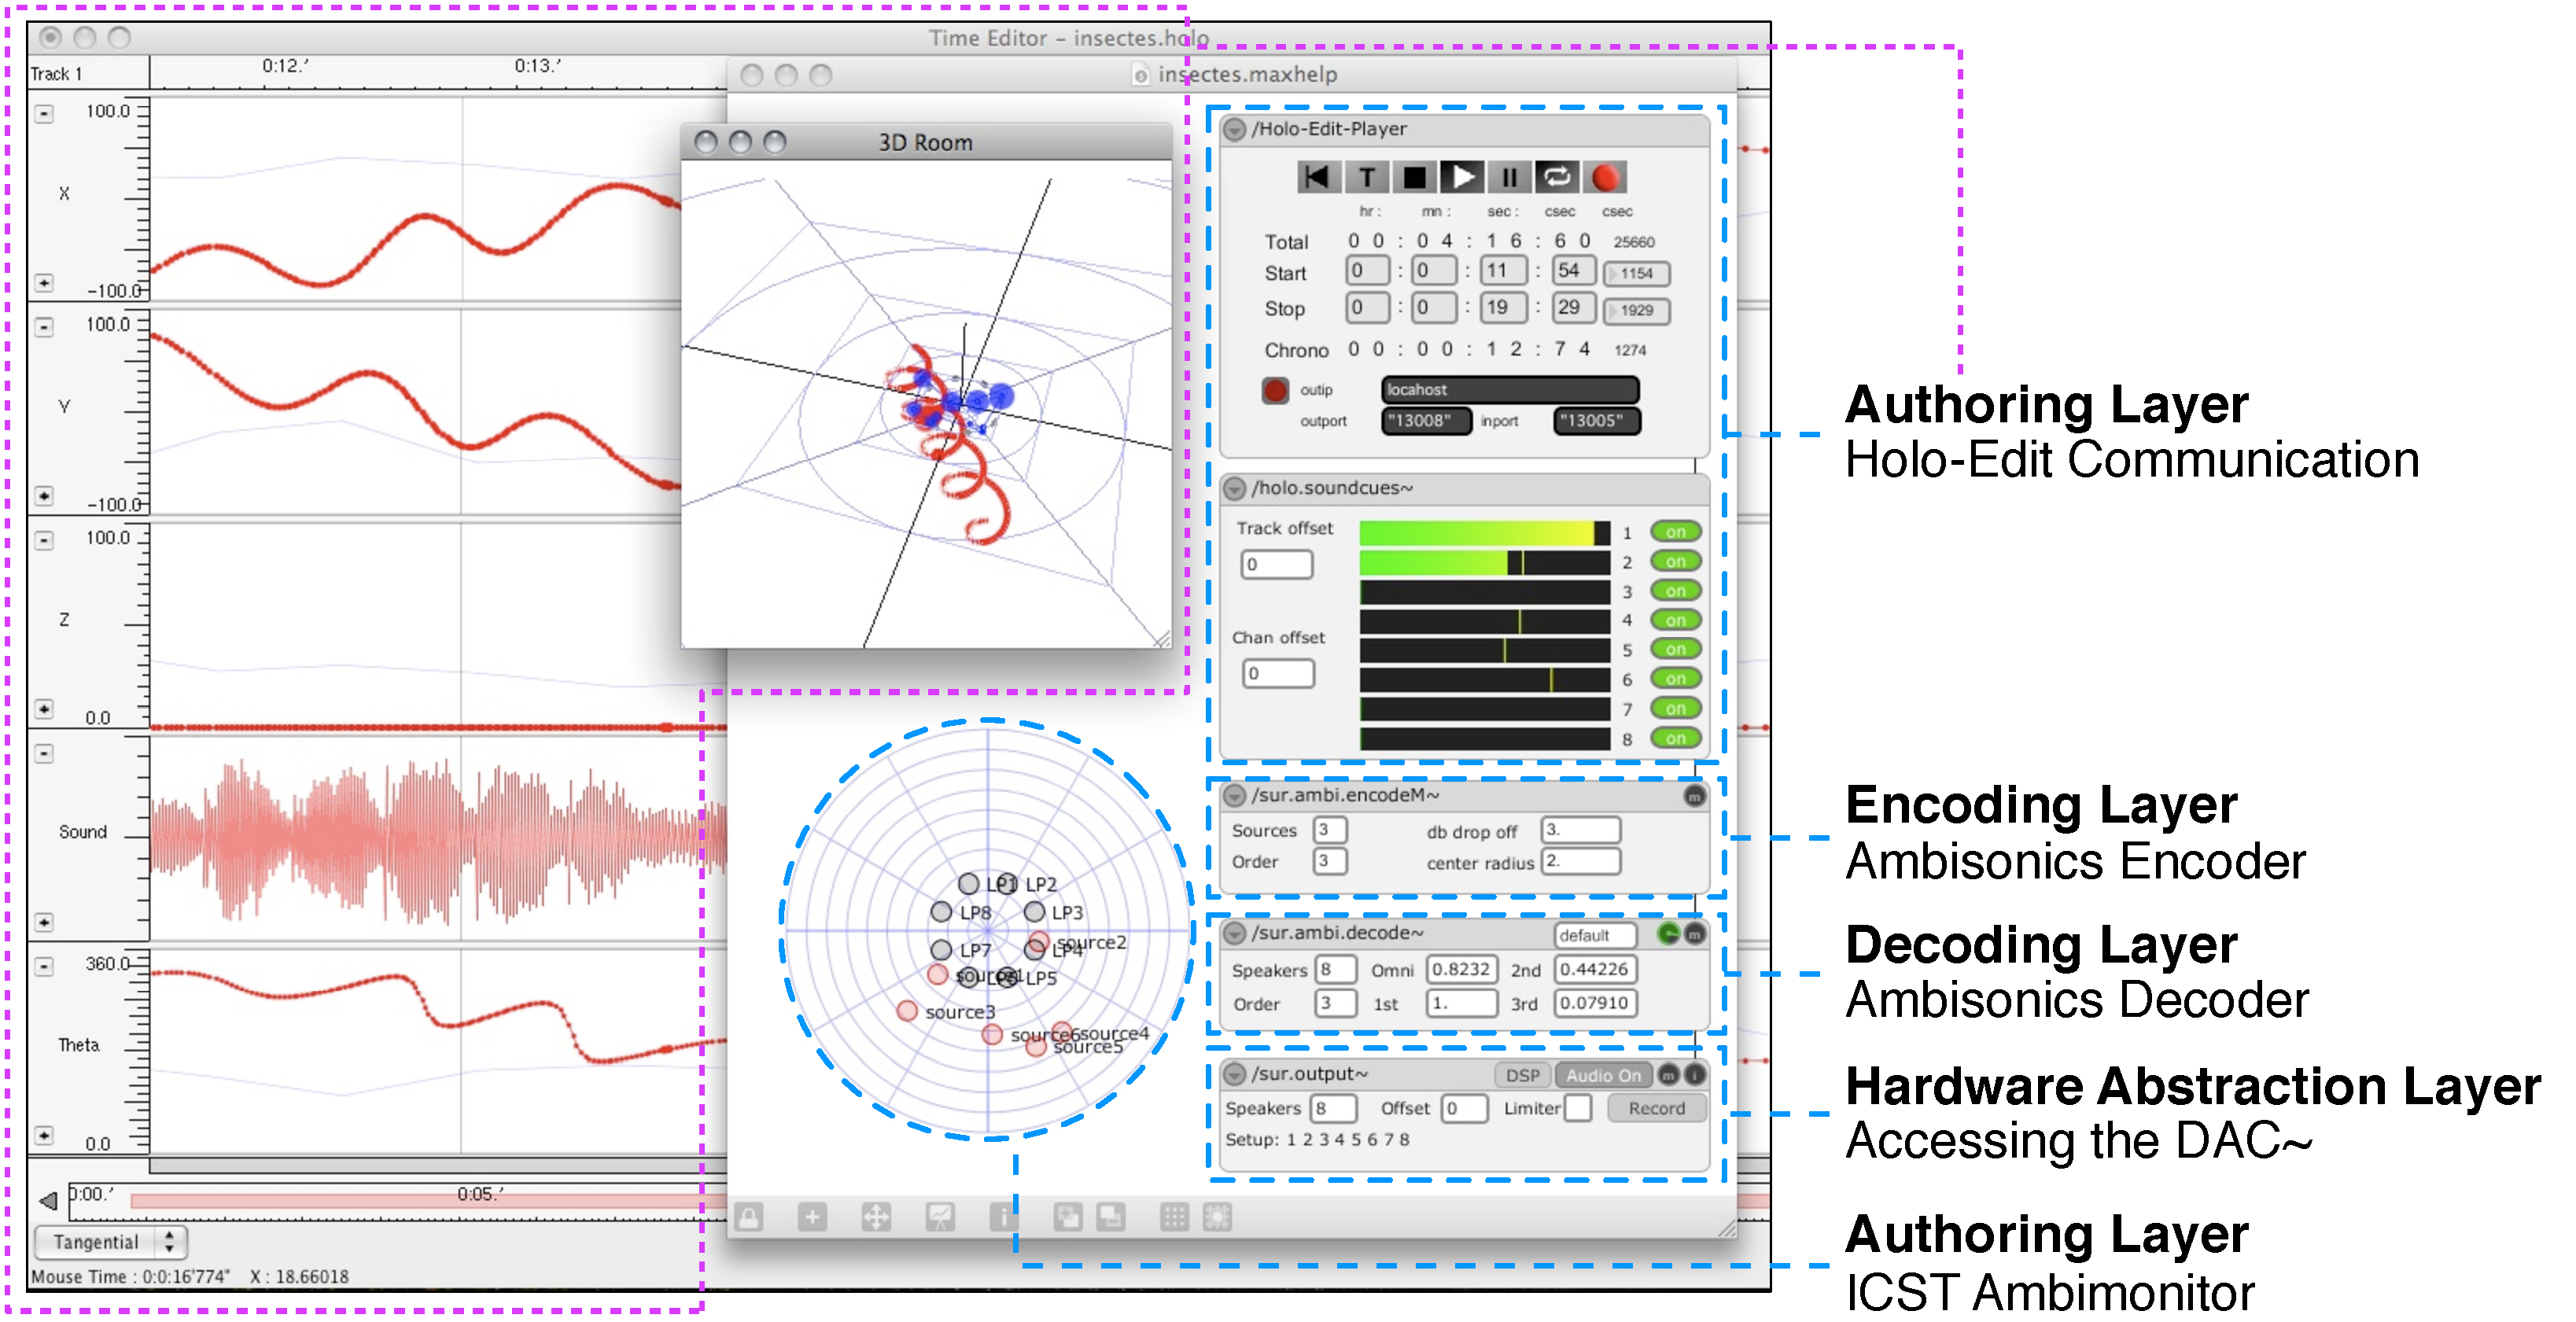
\includegraphics[width=2.2\columnwidth]{smcExample.pdf}} \caption{Holo-Edit, Jamoma and ICST Ambisonics Tools unified} \label{fig:example} 
	\end{figure*}


\section{Discussion \& Conclusion}

%We propose a multi-layer approach to mediate across essential components involved in sound spatialization.
The examples from the previous section illustrate that a stratified model can be fruitful for development within media programming environments. The modular framework TANGA \cite{ReiterTANGA} for interactive audio applications reveals a related separation of tasks.

A few stand-alone applications are designed with a similar layered approach that allows control of different spatial rendering algorithms from one common interface, e.g. \cite{geier2008ssr}. Artists and researchers would benefit greatly if all these ``local solutions" could be accessed by any desired authoring tool and integrated into existing environments.

After an ICMC 2008 panel discussion on interchange formats for spatial audio scenes\footnote{\scriptsize{\url{http://redmine.spatdif.org/wiki/spatdif/Belfast_2008}}} and informal discussion showed that adequate spatialization tools for working in DAWs are missing, but strongly desired. The proposed stratified approach would be more flexible than the current DAW architecture where tools for spatialization are tied to a number of consumer channel configurations. The object oriented mixer approach proposed in \cite{MeltzerTMT08} suggests that stratification can be employed in DAWs. A potential limitation might be imposed by the fact that automation in DAWs generally is represented as time-tagged streams of one-dimensional values while spatial information is generally multi-dimensional.

One keystone may be to define and agree on a meaningful communication format for spatialization. Therefore SpatDIF needs to be further developed which will culminates in an API that easily integrates in any spatialization software.

%
%
%- similar solutions: Mathias, Travis Pope 
%- "Local solution"
%    - importance of interchange communication formats - SpatDIF
%    - further work on SpatDIF - The next step includes developing more use cases and a wider set of tools. SpatDIF and the modular approach to %spatialization needs to grow through implementations in a variety of software, especially commercially used systems DAWs and plugins.
%    - interoperablity only possible to a certain extent, there might be settings that are particular to one rendering technique only. Changing %between them (or from on space to another) will always require a degree of adjusting and adaption.
%    - Integration between Jamoma and HoloEditindicates the potential of cross-platform ....
%
%
%This layered approach is an abstract and simplified description of spatial sound processes. Of course, there are other interacting processes %embedded in a computer music environment, such as the access of memory and hard drives.
%
%
%
%
%By working symbolically during the composition/editing process, and separating the authoring from the rendering processes, a realization can become portable. A common set of descriptors and shared representation metaphors, such as timelines or scene graphs, builds the glue to make a disparate set of tools into a coherent workflow by enhancing interoperability between the building blocks.
%
%
%
%Pope, S. T. and C. Ramakrishnan. �The CREATE Signal Library (�Sizzle�): Design, Issues, and Applications�. Proc ICMC 2003.  See also http://FASTLabInc.com/CSL 
%
%
%%%% Do the following fit in here somewhere?

%\begin{quote}Spatial orchestration eases this [...] constraint, [...] the composition may be reconfigured for each individual performance. This will require [...] the composer [to] conceive spatial attributes in a more abstract fashion that is then instantiated in potentially different ways into different performance environments. \cite{Lyon:2008spatial_orchestration} \end{quote}



%%%%%%%%%%%%%%%%%%%%%%%%%%%%%%%%%%%%%%%%%%%%%%%%%%%%%%%%%%%%%%%%%%%%%%%%%%%%%
%
%%%%%%%%%%%%%%%%%%%%%%%%%%%%%%%%%%%%%%%%%%%%%%%%%%%%%%%%%%%%%%%%%%%%%%%%%%%%%

\section{Acknowledgment}
The concepts proposed in this paper were to a large degree developed during a workshop at GMEA Centre National de Cr\'eation Musicale as part of the Virage research platform funded by the French National Agency for Research. This work is also partly funded by the Canadian Natural Sciences and Engineering Research Council (NSERC), the Canada Council for the Arts, The COST IC0601 Action on Sonic Interaction Design (SID) and the Municipality of Bergen.


\bibliographystyle{abbrv}  %\bibliographystyle{natbib}% ama, nar, alpha, plain, chicago,{plainnat}  abbrv, siam   
\small
\bibliography{smc09}
\end{document}   

%%%%%%%  Poubelle %%%%%%   
	
%\subsection{Frameworks for Spatialization}
%\textbf{Spatialisateur} (Spat) \cite{JotPhD}, in development at IRCAM and Espaces Nouveaux since 1991, is a library of spatialization algorithms for Max/MSP, including VBAP, first-order Ambisonics and stereo techniques (XY, MS, ORTF) for up to 8 loudspeakers. It can also reproduce 3D sound for headphones (binaural) or 2/4 loudspeakers (transaural). A room model is included to create artificial early reflections and reverb controlled by a perceptual-based user interface.\\
%\textbf{Ambisonics toolbox}  \cite{Schacher:2006ambi_max}


% \section{Style Stuff - delme}

% \subsection{Title and Authors}

%The title is 14pt Times, bold, caps, upper case, centered. Authors' names are centered. 
%The lead author's name is to be listed first (left-most), and the co-authors' names after. If the addresses for all 
%authors are the same, include the address only once, centered. If the authors have different addresses, 
%put the addresses, evenly spaced, under each authors' name.

% Reviews are double-blind. {\it \textbf{Author information should be removed from this page in initial submissions}}, 
% and only added later by the authors when sending camera-ready versions.

%\subsection{Figures, Tables and Captions}

%All artwork must be centered, neat, clean, and legible. All lines should
%be very dark for purposes of reproduction and art work should not be hand-drawn.
%The proceedings is not in color, and therefore all figures must make
%sense in black-and-white form.
%Figure and table numbers and captions always appear below the figure. Leave 1
%line space between the figure or table and the caption. Each figure or table
%is numbered consecutively. Captions should be Times 10pt.
%Place tables/figures in text as close to the reference as possible.
%References to figures and tables should be capitalised, for example:
%see Figure \ref{fig:example} and Table \ref{tab:example}.
%Figures and tables may extend across both columns to a maximum
%width of 7'' (17.78~cm).

%\begin{table}
%\begin{center}
%\begin{tabular}{|l|l|}
%\hline
%String value & Numeric value \\
%\hline
%hello SMC  & 1073 \\
%\hline
%\end{tabular}
%\end{center}
%\caption{Table captions should be placed below the table}
%\label{tab:example}
%\end{table}

%\begin{figure}
%\centerline{\framebox{
% To use when using pdflatex
%	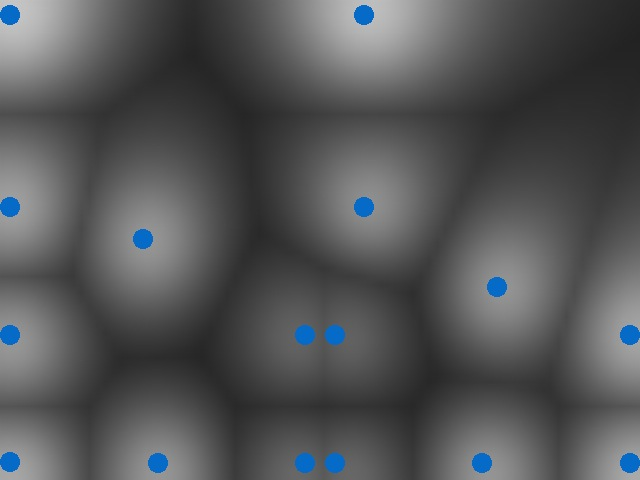
\includegraphics[width=\columnwidth]{../ICMC2009-dbap/all_r_6_b_0_2}}}
	% To use when using latex, dvips and ps2pdf
% 	
\includegraphics[width=\columnwidth]{figure.eps}}}
%\caption{Figure captions should be placed below the figure}
%\label{fig:example}
%\end{figure}